\usepackage[left=2.0cm, 
            right=2.0cm, 
            top=2.0cm, 
            bottom=2.0cm]{geometry} % Настройка геометрии страницы 
\usepackage[utf8]{inputenc} % UTF8 как стандартную кодировку
\usepackage[T2A]{fontenc}
\usepackage[english, russian]{babel} % Поддержка русских и английских особенностей языка
\usepackage{amsmath,amsfonts,amssymb} % Математика
\usepackage{graphicx} % Добавление графики в документ
\usepackage{subfiles} % Поддержка подфайлов
\usepackage{csquotes} 
\usepackage[backend=biber,
            bibencoding=utf8]{biblatex} % https://qna.habr.com/q/484967 % Составление библиографических списков




\begin{document}

\maketitle %создает титульную страницу

\frontmatter % выключает нумерацию ВСЕГО; здесь начинаются ненумерованные главы: реферат, введение, глоссарий, сокращения и прочее.







% \listoffigures                         % Список рисунков

% \listoftables                          % Список таблиц

%\NormRefs % Нормативные ссылки
% Команды \breakingbeforechapters и \nonbreakingbeforechapters
% управляют разрывом страницы перед главами.
% По-умолчанию страница разрывается.

% \nobreakingbeforechapters
% \breakingbeforechapters

% 
Титульный лист 

Список исполнителей


% Также можно использовать \Referat, как в оригинале
\begin{Referat}

    \pageref{LastPage}\,стр.%
    \ifnum \totfig >0 , \totfig~рис.%
    \fi
    \ifnum \tottab >0 , \tottab~табл.%
    \fi
    %
    \ifnum \totbib >0 , \totbib~источн.%
    \fi
    %
    \ifnum \totapp >0 , \totapp~прил.%
    \else
    .%
    \fi

    ИДЕНТИФИКАЦИЯ СИСТЕМ, НЕЙРОННЫЕ СЕТИ, МОДЕЛИРОВАНИЕ ПРОЦЕССОВ, ПРОГРАММНЫЕ
    СРЕДСТВА ИДЕНТИФИКАЦИИ, ВЫЧИСЛИТЕЛЬНЫЕ СИСТЕМЫ.

    Тема выпускной квалификационной работы: <<Разработка алгоритмов и программ
    динамической идентификации энергетического объекта>>.

    Данная работа посвящена разработке и применению метода динамической
    идентификации сложных промышленных систем с использованием декомпозиционного
    подхода и нейронных сетей. Основной целью исследования является создание
    эффективного инструмента для построения цифровых двойников многокомпонентных
    систем, обеспечивающего высокую точность моделирования и упрощение процесса
    идентификации. Работа охватывает теоретические основы, разработку
    программного обеспечения и практическую апробацию предложенного метода на
    примере теплоэнергетического объекта — парового котла ГМ-50. 
    \nocite{*}

\end{Referat}

%%% Local Variables: %% mode: latex %% TeX-master: "rpz" %% End: 


\begin{ReferatEng}

    \pageref{LastPage}\,p.%
    \ifnum \totfig >0 , \totfig~fig.%
    \fi
    \ifnum \tottab >0 , \tottab~tab.%
    \fi
    %
    \ifnum \totbib >0 , \totbib~ref.%
    \fi
    %
    \ifnum \totapp >0 , \totapp~app.%
    \else
    .%
    \fi

    SYSTEM IDENTIFICATION, NEURAL NETWORKS, PROCESS MODELING, IDENTIFICATION
    SOFTWARE TOOLS, COMPUTATIONAL SYSTEMS.

    The subject of the graduate qualification work is <<Development of
    algorithms and software for dynamic identification of an energy facility>>.

    This study focuses on the development and application of a dynamic
    identification method for complex industrial systems using a decompositional
    approach and neural networks. The primary objective of the research is to
    create an effective tool for building digital twins of multicomponent
    systems, ensuring high modeling accuracy and simplifying the identification
    process. The work covers theoretical foundations, software development, and
    practical validation of the proposed method, demonstrated on a thermal power
    facility—the GM-50 steam boiler.

\end{ReferatEng}


\tableofcontents

% \printnomenclature % Автоматический список сокращений

Вступление


\mainmatter % это включает нумерацию глав и секций в документе ниже


% Теоретическая часть
\chapter{Теоретическая часть}


% Техническая часть
\chapter{Программные средства технологических промышленных систем}



\section{Работа с нейронными сетями}

Развитие и применение нейронных сетей в задачах
динамической идентификации, неразрывно связано с
наличием мощных и гибких программных инструментов.
Эти инструменты предоставляют необходимые библиотеки
и фреймворки для создания архитектур нейронных
сетей, эффективного обучения на больших объемах
данных, в том числе с использованием специального
оборудования, например, графические процессоры GPU
или матричные процессоры TPU, и последующего
развертывания разработанных моделей. Выбор
соответствующего программного стека имеет
критическое значение для продуктивности
исследования, масштабируемости решений и возможности
воспроизведения результатов.

\subsection{Язык программирования}

Развитие инструментов для работы с нейронными сетями было неразрывно с
развитием языков и библиотек, нацеленных на высоконагруженные вычисления - C и
Fortran. Со временем, количество исследователей и пользователей увеличивалось и
развитие данных инструментов сместилось в область <<удобства>> пользования. В
частности, за последние гда выделилось множество языков, определивших базисный
инструментарий для работы с нейронными сетями. К языкам, активно используемых в
области машинного обучения и разработки нейронных сетей и составляющим этот
базис, можно отнести несколько языков программирования:

\begin{itemize}
  \item Python;
  \item MATLAB;
  \item R;
  \item C++;
  \item Julia.
\end{itemize}

\subsubsection{Python}
Python является интерпретируемым языком и особенно популярен в области науки о
данных и машинного обучения. Он обладает простым синтаксисом, обширной
экосистемой библиотек для научных вычислений и визуализации, а также большим
количеством высокопроизводительных фреймворков для глубокого обучения. Также,
язык поддерживает множество инструментов для создания графических
пользовательских интерфейсов. Его универсальность и легкость интеграции с
другими языками делают его привлекательным для полного цикла исследования — от
предобработки данных до построения и тестирования моделей. Также, несмотря на
интерпретируемость, большинство библиотек написаны на C, что позволяет
преодолеть проблемы с низкой производительностью интерпретатора. Кроме того,
решения на Python зачастую являются кросс-платформенными, что расширяет
возможности проектов для масштабирования и расширения. 

\subsubsection{MATLAB} 
MATLAB является пакетом для математических вычислений, включающий в себя
большое количество различных пакетов, предоставляет интегрированную среду
разработки и набор специализированных тулбоксов, в том числе для нейронных
сетей и глубокого обучения. Пакет реализует одноименный язык для написания
скриптов, основной особенностью которого является уклон в стороную простоты
написания и математической формализации.

Несмотря на широкий круг возможностей, он является коммерческим продуктом, что
может ограничивать доступность, и его экосистема библиотек, хотя и обширна в
своей нише, менее открыта и широка по сравнению с Python для самых передовых
исследований в области глубокого обучения. Кроме того, скрипты ограничены
окружением MATLAB и может быть переиспользованы обособлено.

\subsubsection{R}

R – это язык статистических вычислений и анализа данных с открытым исходным
кодом, созданный для работы с большими объемами данных, визуализации и
статистического моделирования. Имеет широкий спектр возможностей, включая
статистику данных, машинное обучение, визуализацию данных и т.д. Однако, язык
имеет неполную поддержку библиотек для работы с нейронными сетями и показывает
плохую производительность.

\subsubsection{C++} 
C++ является компилируемым языком общего назначения с высокой производительностью,
часто используемый для системного программирования и высоконагруженных
вычислений. Несмотря на высокую производительность и наличие библиотек, в
последние года их поддержка прекратилась и язык стал все реже использоваться в
проектах. Кроме того, сложность написания кода при работе с библиотеками и
высокому <<уровню входа>> в язык привела к оттоку разработчиков и переходу их
на Python.

\subsubsection{Julia} 
Julia – это высокоуровневый язык для научных вычислений, сочетающий скорость C++ с удобством Python и R. Язык имеет широкий список встроенных пакетов для научных вычислений и их ускорения, в том числе и с помощью параллелизации и графических ускорителей. Однако, язык относительно молодой и не имеет широкого стабильного инструментария для машинного обучения и в частности нейронных сетей. Кроме того, отсутствуют инструменты для раздработки оконных интерфейсов. 

Исходя из всех вышеописанных особенностей каждого из языков очевидно, что наиболее предпочтительным для разработки как модели для динамической идентификации, так и разработки для неё инструментов с оконным интерфейсом, наиболее всего подходит язык Python.

\subsection{Фреймворк}

Язык Python имеет множество библиотек, реализующих различные модели нейронных
сетей, а также алгоритмов машинного обучения. К таковым относятся как простые
библиотеки, предназначенные для изучения и обучения, так и промышленные
библиотеки, предназначенные для оптимальной и эффективной раброты с нейронными
сетями. Среди них особенно выделяются следующие библиотеки:

\begin{itemize}
  \item JAX;
  \item Tensorflow;
  \item PyTorch. 
\end{itemize}

\subsubsection{Tensorflow}

TensorFlow — фреймворк с открытым исходным кодом для построения и обучения
нейронных сетей. Поддерживает статические и динамические графы вычислений.
Интегрирован с библиотекой Keras, обеспечивающей более высокоуровневое API. 

Основным преимуществом данной библиотеки является реализация на C++,
обеспечивающая наибольшую скорость выполнения среди всех остальных библиотек.
Библиотека поддерживает все виды моделей и позволяет переносить и
переиспользовать обученные модели. 

\subsubsection{PyTorch}

PyTorch - это библиотека с открытым исходным кодом для работы с нейронными
сетями. Библиотека имеет реализацию на Python, в связи с чем её работа
обусловлена низкой скоростью. Библиотека имеет простой синтаксис и имеет малый
порог входа для начала работы. 

Библиотека имеет встроенные модули для работы с данными, а также встроенный
высокоуровневый API. Также, PyTorch поддерживает построение динамических графов
расчетов, что позволяет <<отлаживать>> обучение модели. 

Однако, в связи с малой скоростью работы, библиотека только используется в академических задачах. 

\subsubsection{JAX}

JAX является библиотекой для изучения нейронных сетей, объединяющая особенности
как PyTorch, так и Tensorflow, однако в связи с тем, что библиотека нова, имеет
плохую документацию и недостаточно описана. JAX имеет высокую
производительность, однако содержит меньше готовых компонентов и моделей для
разработки нейросетей. 

В соответствии с производительностью библиотек и возможностью интеграции с другими модулями, Tensorflow с модулем Keras является наиболее предпочтительным для работы в задаче динамической идентификации. 

\section{Инструменты создания оконных интерфейсов}

Инструментарий языка Python содержит широкий спектр библиотек, в том числе, обеспечивающих создание графических пользовательских интерфейсов. 
Наиболее часто используемыми библиотеками являются следующие

\begin{itemize}
  \item Tkinter;
  \item PyQt.
\end{itemize}


\subsection{Tkinter}

Tkinter - это простая встроенная библиотека Python
для создания базовых элементов GUI, часто
используемая для небольших проектов или быстрого
прототипирования. 

Библиотека включена в стандартную библиотеку Python
(начиная с версии 3.x), что делает его наиболее
доступным инструментом для создания
кроссплатформенных десктопных приложений. Tkinter
предоставляет объектно-ориентированный интерфейс для
работы с элементами управления (виджетами) и
поддерживает модель событийно-ориентированного
программирования.

Недостатком Tkinter является невозможность создания пользовательских компонентов, что сильно ограничивает разработку сложных интерфейсов.

\subsection{PyQt}

PyQt - это кроссплатформенный GUI-фреймворк,
предоставляющий богатый набор виджетов и
инструментов для создания визуально привлекательных
и интерактивных приложений на Python.

Кроссплатформенность PyQt позволяет разрабатываемому
программному обеспечению работать на различных
операционных системах, обеспечивая более широкую
доступность. Он предлагает обширную коллекцию
готовых виджетов и инструментов для создания сложных
и удобных графических интерфейсов.142 PyQt тесно
интегрирован с Python, что позволяет разработчикам
беспрепятственно сочетать GUI с логикой приложения и
моделями машинного обучения.

PyQt выделяется как сильный выбор для разработки GUI благодаря сочетанию кроссплатформенной совместимости, богатого набора функций для создания сложных интерфейсов, бесшовной интеграции с Python и производительности, обеспечиваемой его основой на языке C++.



% Практическая часть
\chapter{Разработка алгоритмов и средств динамической идентификации}
%TODO
 
\section{Описание исследуемого объекта}
%TODO: Добавить описание котельного агрегата, базы данных

\section{Выбор архитектуры нейронных сетей}

Появление методов глубокого обучения привели к появлекнию множества различных архитектур нейронных сетей, в частности их компонентов. Архитектура нейронной сети во многом определяется классом задачи и её правильный выбор необходимо делать исходя из особенностей данных и желаемого результата. Несмотря на широкий спектр задач, которые решают те или иные архитектуры, не все модели подходят для решения задач идентификации.

\subsection{Полносвязная нейронная сеть}

Полносвязанные нейронные сети — это нейронные сети, в которых каждый 
нейрон передает свой выходной сигнал остальным нейронам, в том числе 
и самому себе. 

\begin{figure}[H]
  \centering
    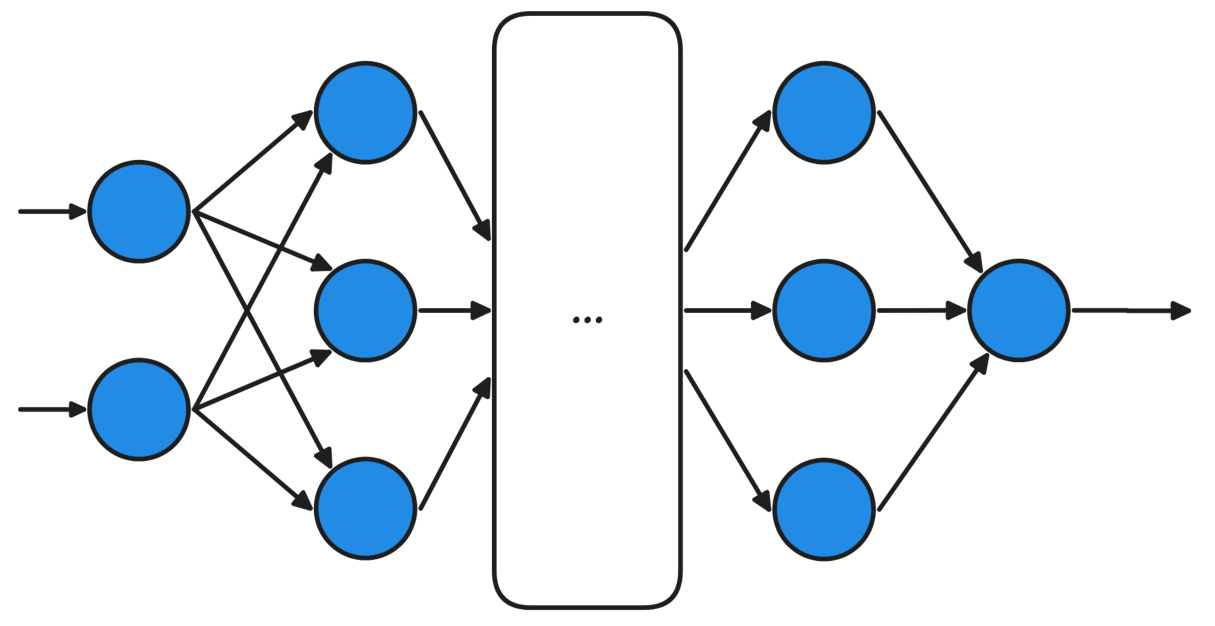
\includegraphics[width=0.9\textwidth]{figures/arch_fully_connected.png}
  \caption{Архитектура полносвязной сети}\label{fig:dense_nn}
\end{figure}

Все входные сигналы подаются всем нейронам, находящимся 
на текущем слое (см. рис. \ref{fig:dense_nn}). Выходными сигналами сети могут быть все или некоторые
выходные сигналы нейронов.

Такие модели могут использоваться для аппроксимации сложных многомерных
функций, представляющих множество целей оптимизации. Часто применяются для
построения суррогатных моделей для оценки функций без необходимости прямого
вычисления.

\subsection{Рекуррентная нейронная сеть}

Рекуррентная нейронная сеть — это тип искусственных нейронных сетей, широко
используемый для обработки последовательных данных и временных рядов. 

\begin{figure}[H]
  \centering
    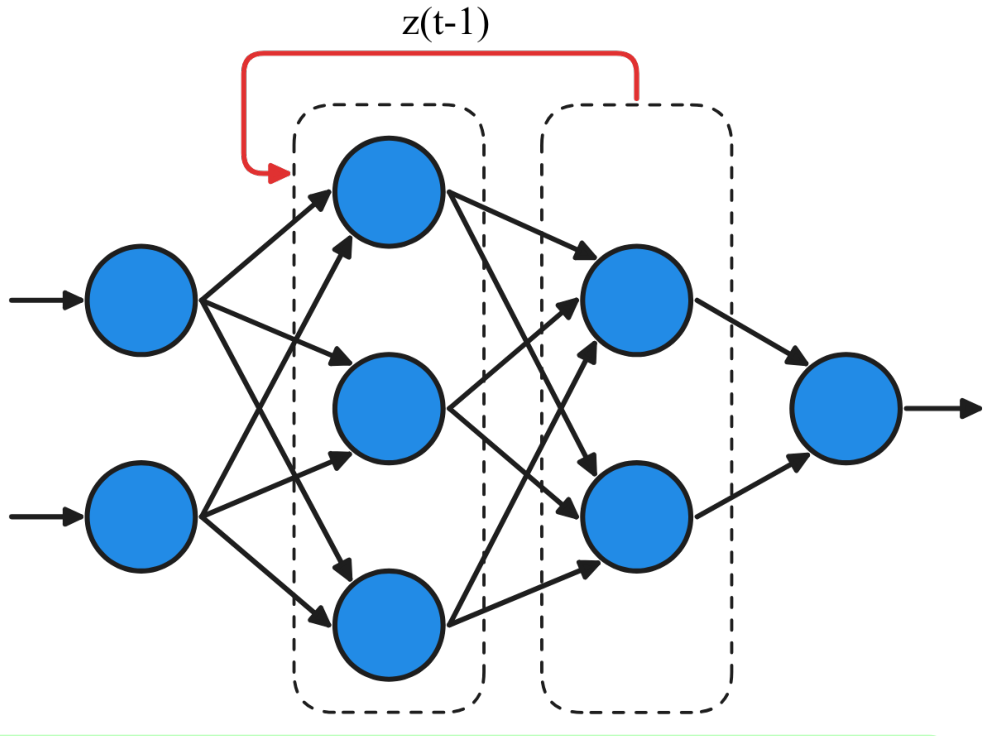
\includegraphics[width=0.9\textwidth]{figures/arch_rnn.png}
  \caption{Архитектура рекуррентной сети}\label{fig:rnn}
\end{figure}

В отличие от традиционных нейронных сетей, например, многослойных перцептронов, где
обработка данных происходит только в одном направлении, RNN имеют петли (см.
рис. \ref{fig:rnn}). Эти петли позволяют сохранять и использовать информацию из 
предыдущих состояний сети, что делает RNN особенно полезными для задач, где важен 
контекст и зависимость данных во времени. 

В задачах динамической идентификации, где необходимо учитывать не только прямые
связи систем, но также и краевые эффекты, оказывающие влияние на смежные
системы, RNN могут быть полезны благодаря своей способности учитывать контекст
и исторические данные.

\subsection{Сверточная нейронная сеть}

Сверточная нейронная сеть — особый тип нейронной сети, основанный на
полносвязной сети и имеющий как минимум один особый сверточный слой. 

\begin{figure}[H]
  \centering
    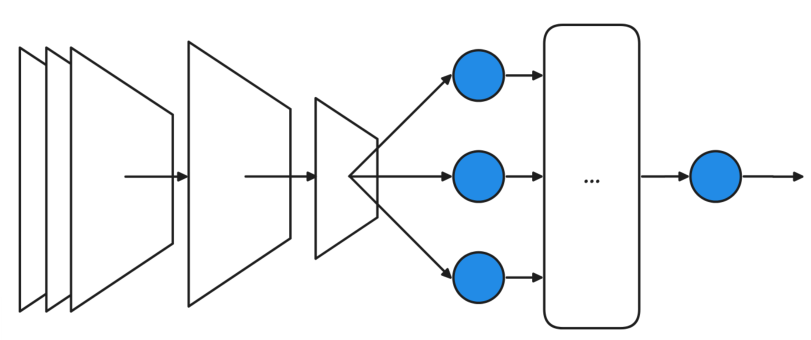
\includegraphics[width=0.9\textwidth]{figures/arch_cnn.png}
  \caption{Архитектура сверточной сети}\label{fig:cnn}
\end{figure}

Сверточный слой — нейронный слой, позволяющий производить понижение или повышение
размерности данных. Из-за своей особой архитектуры (см. рис. \ref{fig:cnn}),
сети позволяют эффективно обрабатывать данные с пространственной структурой.

Данная категория нейронных сетей применяется в случаях, если входы системы
имеют пространственную структуру, в которой элементы связанны между собой. Они
применяются для обнаружения признаков или шаблонов, влияющих на общую работу
системы.

Зачастую данный тип нейронных сетей используется в связи с другими
архитектурами, предоставляя им возможности работы с небольшими данными с
выделенными общими признаками.

\subsection{Автокодировочная нейронная сеть}

Автокодировщик — это тип нейронной сети, используемой для обучения эффективного
кодирования данных. Цель автокодировщика — научиться представлять входные
данные в более сжатом и информативном виде, называемом латентным пространством,
и затем восстанавливать оригинальные данные из этого представления. 
\begin{figure}[H]
  \centering
    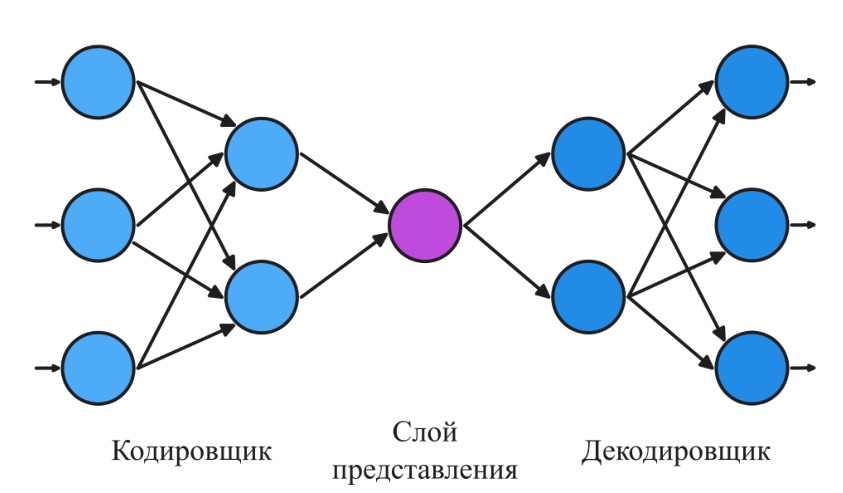
\includegraphics[width=0.9\textwidth]{figures/arch_autoencoder.png}
  \caption{Архитектура сети-автокодировщика}\label{fig:autoencoder}
\end{figure}

Он состоит из двух основных частей: энкодера и декодера (см. рис.
\ref{fig:autoencoder}). Энкодер преобразует входные данные в сжатое 
скрытое представление (латентное пространство), а декодер восстанавливает 
исходные данные из этого представления. Задача декодера — восстановить данные 
из их скрытого сжатого представления. Данный тип моделей позволяет находить 
компактные представления данных и выявлять скрытые закономерности в них.
В некоторых типах автокодировщиков добавляют вероятностную интерпретацию, что
позволяет моделировать неопределенности в данных и оптимизировать несколько
целей одновременно через латентное пространство.

Архитектурные особенности автокодировщиков не предполагают использования их в
качестве моделей, описывающих системы, однако могут использоваться с целью
повторения помех в данных и приближения их к реальным.

\subsection{Сравнение архитектур}
%TODO: Описание тестового набора

Для того, чтобы сравнить производительность различных архитектур нейронных
сетей выберем из рассмотренного ранее набора данных набор связанных параметров
и произведем для выбранной подсистемы построение цифрового двойника. 

В качестве исследуемых параметров выберем систему с одним входным и выходным
параметром - нагревательный котел. В качестве входного параметра выберем
массовый расход мазута, а выходным температура в котле. Соответственно,
повышение мазута, поступающего на нагрев котла, должно приводить к повышению
температуры внутри котла. 

\begin{figure}[H]
  \centering
    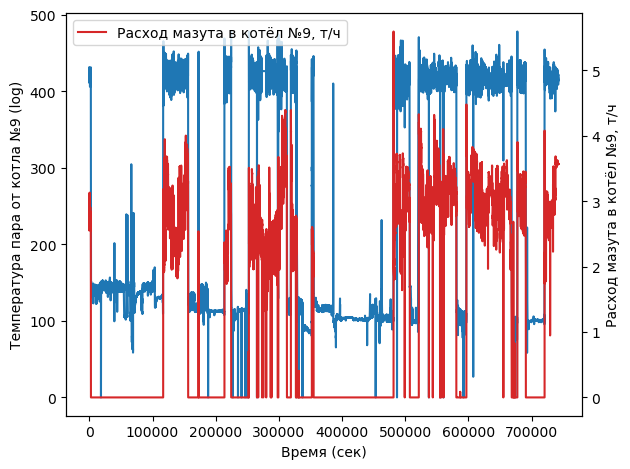
\includegraphics[width=0.85\textwidth]{figures/plots/kotel_temp_mazut.png}
  \caption{Временные характеристики параметров котла}\label{fig:plt:kotel}
\end{figure}

Из временных зависимости входного и выходного параметров (см. рис.
\ref{fig:plt:kotel}) видно, что параметры имеют связь. 

\begin{figure}[H]
  \begin{center}
    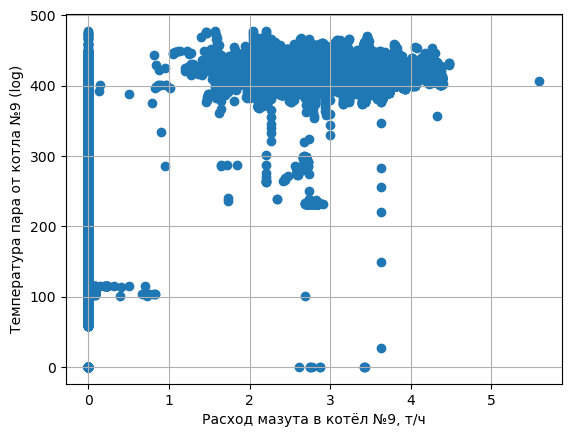
\includegraphics[width=0.85\textwidth]{figures/plots/kotel_temp_mazut_rel.png}
  \end{center}
  \caption{Корреляция между параметрами котла}\label{fig:plt:kotel:rel}
\end{figure}

Из построения характеристики между параметрами (см. рис.
\ref{fig:plt:kotel:rel}) видно, что характер зависимости не является
линейным и трудно описываем простыми выражениями. 

\subsubsection{Полносвязная сеть}

Произведем идентификацию с помощью многослойной
нейронной сети. 

\begin{figure}[H]
  \begin{center}
    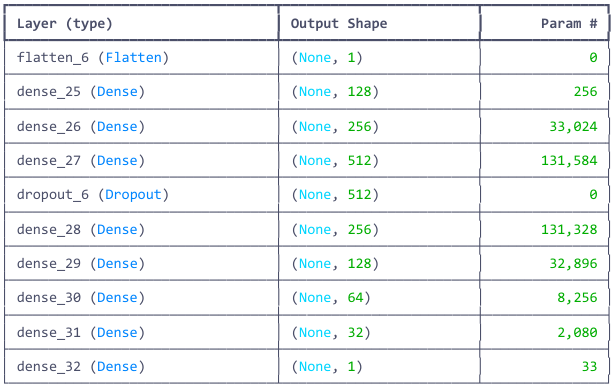
\includegraphics[width=0.95\textwidth]{figures/tensorflow/dense.png}
  \end{center}
  \caption{Конфигурация полносвязной сети}\label{fig:tf:dense}
\end{figure}

Архитектура сети выбрана исходя условия отсутствия
сужений относительно количества входов и выходов (см.
рис. \ref{fig:tf:dense}). 

Обучение производится на 50 эпохах с учетом
разделения данных на $80\%$ на обучающую выборку и
$20\%$ тестирование и валидацию. 

\begin{figure}[H]
  \begin{center}
    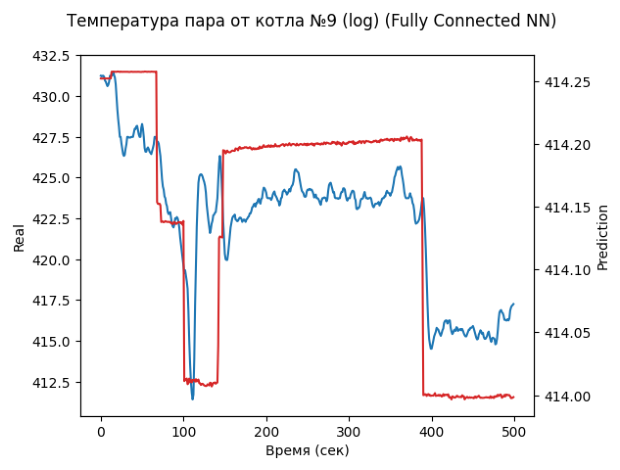
\includegraphics[width=0.95\textwidth]{figures/tensorflow/dense_compare.png}
  \end{center}
  \caption{Сравнение полученной модели полносвязной нейронной сетью}\label{fig:tf:cmp:dense}
\end{figure}

Из полученных результатов (см. рис. \ref{fig:tf:cmp:dense}) можно видеть, что
общая динамика системы повторяется, кроме того, нейтрализуются всплески,
обусловленные шумом. 

\subsubsection{Рекуррентная сеть}

Произведем идентификацию с помощью рекуррентной
нейронной сети. 

\begin{figure}[H]
  \begin{center}
    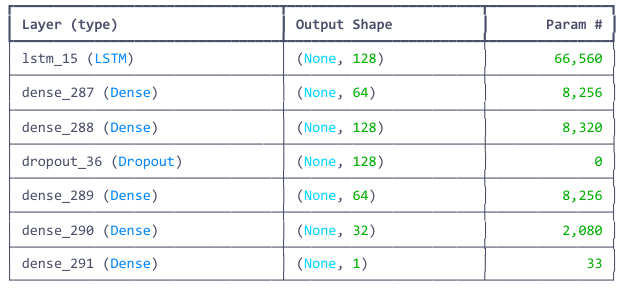
\includegraphics[width=0.95\textwidth]{figures/tensorflow/rnn.png}
  \end{center}
  \caption{Конфигурация рекуррентной сети}\label{fig:tf:rnn}
\end{figure}

Архитектура сети выбрана исходя условия отсутствия
сужений относительно количества входов и выходов (см.
рис. \ref{fig:tf:rnn}). 

Обучение будем производить с теми же свойствами, что и предыдущую. 

\begin{figure}[H]
  \begin{center}
    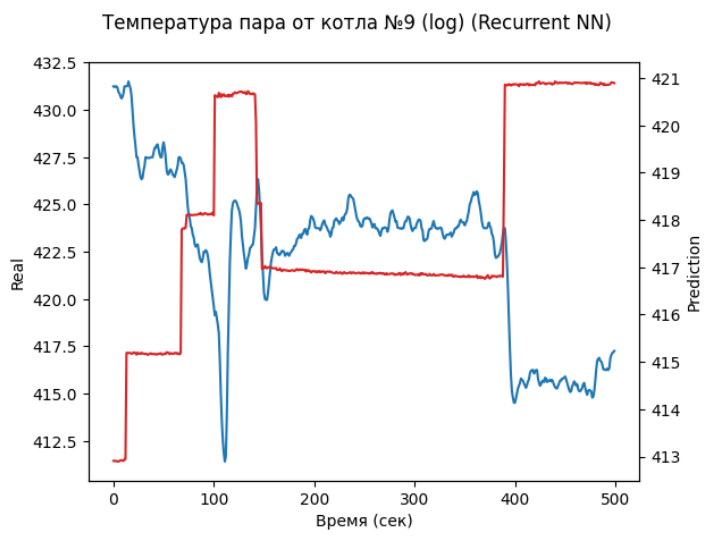
\includegraphics[width=0.95\textwidth]{figures/tensorflow/rnn_compare.png}
  \end{center}
  \caption{Сравнение полученной модели рекуррентной нейронной
  сетью}\label{fig:tf:cmp:rnn}
\end{figure}

Из полученных результатов (см. рис. \ref{fig:tf:cmp:rnn}) можно видеть, что
общая динамика системы повторяется, кроме того, нейтрализуются всплески,
обусловленные шумом, однако выход сети перевернут. 

\begin{figure}[H]
  \begin{center}
    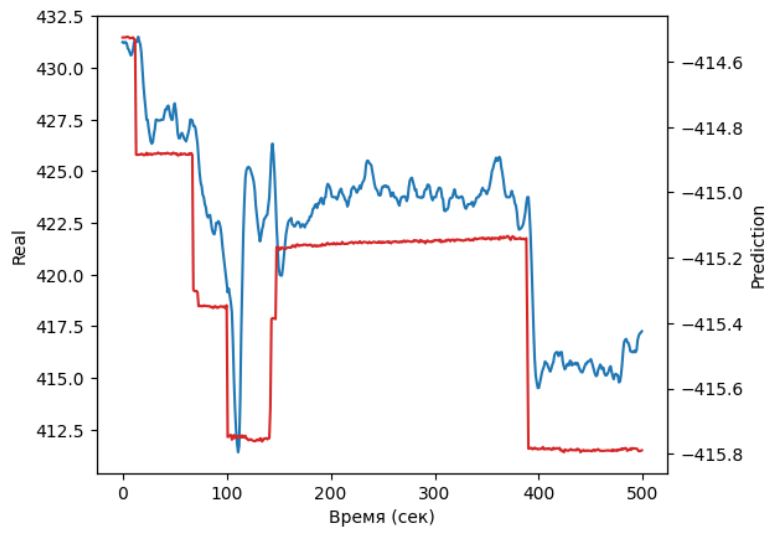
\includegraphics[width=0.95\textwidth]{figures/tensorflow/rnn_compare_reversed.png}
  \end{center}
  \caption{Сравнение полученной модели рекуррентной нейронной
  сетью}\label{fig:tf:cmp:rnn:reversed}
\end{figure}

С учетом переворота графика получаем, что метод имеет меньшую статическую
ошибку нежели полносвязная сеть (см. рис. \ref{fig:tf:cmp:rnn:reversed}).

Однако, реккурентная сеть позволяет получать только следующие значения,
основываясь на последовательностях. Для идентификации, основывающейся на
фактических параметрах модели лучшен использовать полносвязную сеть, наиболее подробно повторяющую динамику системы. 

\section{Декомпозиционный метод идентификации нейронными сетями}
%TODO: Описание предлагаемого метода
Большинство методов идентификации предполагают создание общей модели в виде
<<черного ящика>>, однако для многих больших систем такое моделирование, в
случае наличия дополнительных данных о внутренних сигналах, может быть
неэффективно. Причиной для этого может служить упущением данных о внутренней
структуре или подсистемах, взаимодействующих друг с другом и оказывающих
влияние на общий результат. Кроме того, зачастую необходимо учитывать значение
параметров подсистем при определенных режимах работы.

Точность идентификации во многом зависит от сложности рассматриваемой системы.
Малые системы дают более точный результат при меньшей сложности создания модели
или обучении нейронной сети. Из этого можно сделать вывод, что точность
построения цифрового двойника во многом связана с размером моделируемой
системы, чем меньше система, тем проще её описать. 

В связи с этим, предлагается непараметрический метод идентификации с
использованием связанного множества нейронных сетей, представляющих подсистемы
общей системы. Каждая рассматриваемая нейронная сеть иммитирует поведение
каждой своей подсистемы. При этом всём важно обеспечить связь между
подсистемами для моделирования все системы в целом. Для этого необходимо
соотвествтующее программное обеспечение, которое бы позволяло производить
полный цикл действий по динамической идентификации предложенным методом. 

\section{Программное обеспечение динамической идентификации}
%TODO: Привести информацию о наличии других ПО для моделирования
%       и то, что зачастую сложные методы поставляются с использованием замкнутого цикла ПО

Разработка удобного графического интерфейса, наиболее полно расрывающего
возможности предлагаемого решения для пользователья, сложный процесс, требующий
точного и скурпулёзного проектирования. В рамках разработки важными этапами
являются:

\begin{itemize}
  \item Выделение требований к разрабатываемой системе;
  \item Определение паттернов и структур данных;
  \item Реализация интерфейса;
  \item Оценка работы системы.
\end{itemize}

\subsection{Требования к системе}
%TODO: Привести требования к предлагаемому ПО

Выделение требований один из наиважнейших этапов, который выделяет необходимые требования и возможности будущего приложения. В рамках разработки приложения для реализации предложенного метода идентификации были выделены следующие требования:

\begin{itemize}
  \item Создавать или загружать данные о сигналах;
  \item Конфигурировать системы с заданным именем, входными и выходными
    сигналами;
  \item Объединять созданные подсистемы в единую связанную систему в
    соответствии с параметрами, определенными пользователем;
  \item Задавать параметры обучения для каждой системы;
  \item Отображать созданную систему в виде связанного графа;
  \item Позволять вручную вводить значения для каждого из сигналов;
  \item Сохранять параметры систем и их иерархию в виде файлов.
\end{itemize}

Все выше перечисленные возможности должны быть реализованы в рамках одного приложения.


\subsection{Структуры данных}
%TODO: Какие структуры данных, их иерархия, паттерны использовались
Основой любого приложения являются данные. Правильный выбор абстракций и определение необходимых структур данных на начальном этапе разработке играет большую роль, определяющую такие свойства приложения как масштабируемость приложения с возможностью расширения функциональных возможностей. 

Кроме того, важно выбрать паттерны проектирования, позволяющие работать с большим количеством объектов. 

В рамках анализа базовых компонентов было выделено 2 основных базовых класса: 

\begin{itemize}
  \item Связь (Connection);
  \item Система (System). 
\end{itemize}

\subsubsection{Класс <<Связь>>}

Класс связи (Connection) предназначен для реализации связывания подсистем и процессов, протекающих между системами. 

Класс также обеспечивает возможности передачи сведений от одной системы к другой (значений сигналов). 

Каждый сигнал уникален и не повторяет по имени никакой другой.

\subsubsection{Класс <<Система>>}

Класс системы (System) предназначен для абстракции данных, связанных с
какой-либо подсистемой. Он содержит информацию о сигналах, являющихся входными
или выходными. Также, он содержит информацию о модели нейронной сети,
аппроксимирующей её поведение. 

Каждая система должна удовлетворять критерию уникальности и не быть дубликатом
другой системы. 

\subsubsection{Менеджеры классов}

Для корректного использования объектов систем и сигналов
реализованы классы, управляющие созданием и изменением объектов данного
класса – менеджеры. 

Каждый класс-менеджер, ConnectionManager и SystemManager, реализует паттерны
Singleton и Abstract Factory - в рамках всего приложения менеджеры уникальны и
учитывают созданные в текущей сессии системы и связи. 

Также, менеджеры обеспечивают учет связей между компонентами, помня какой
сигнал с какой системой связан, позволяя получать граф связей без необходимости
обхода всей системы.

\subsubsection{Вспомогательные классы}

Для поддержания абстракций реализован класс аппроксиматор, реализуйющий
создание и обучение нейронной сети для конкретной заданной системы -
SystemNeuralModel. Любые действия, связанные с идентификационной моделью,
включая создание, обучение или моделирование, выполняется через него. 

\begin{figure}[H]
  \begin{center}
    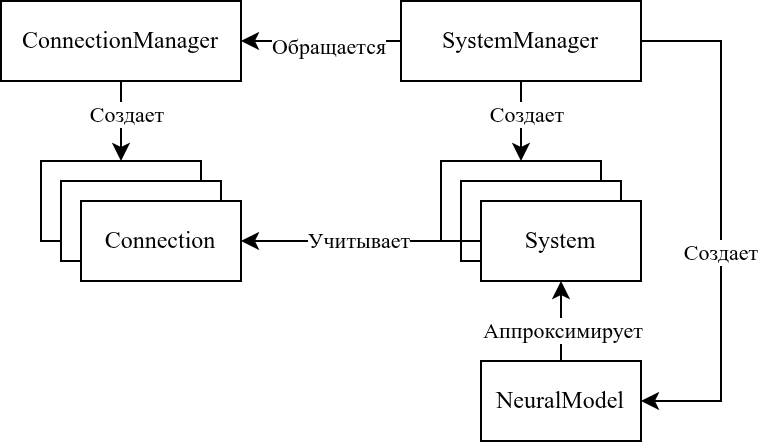
\includegraphics[width=0.95\textwidth]{figures/basics_relations.png}
  \end{center}
  \caption{Взаимодействие базовых компонент системы}\label{fig:basics:components}
\end{figure}

Каждый из классов (см. рис. \ref{fig:basics:components}) работает в связи с другими и реализует базовый функционал для конфигурации исследуемых сигналов и систем.

\subsection{Архитектура приложения}
%TODO: Привести список компонентов, их назначение и связь между собой

Программное обечпечение реализует возможности проведения процесса динамической идентификации, обеспечивая следующих возможности:
\begin{itemize}
  \item Компановка структуры сигналов и систем;
  \item Обучение моделей на базе нейронных сетей;
  \item Моделирование процессов системы.
\end{itemize}

Для обеспечения выполнения перечисленных возможностей, программное обеспечение состоит из нескольких ключевых компонентов, обеспечивающих функциональность динамической идентификации. 

\begin{figure}[H]
  \begin{center}
    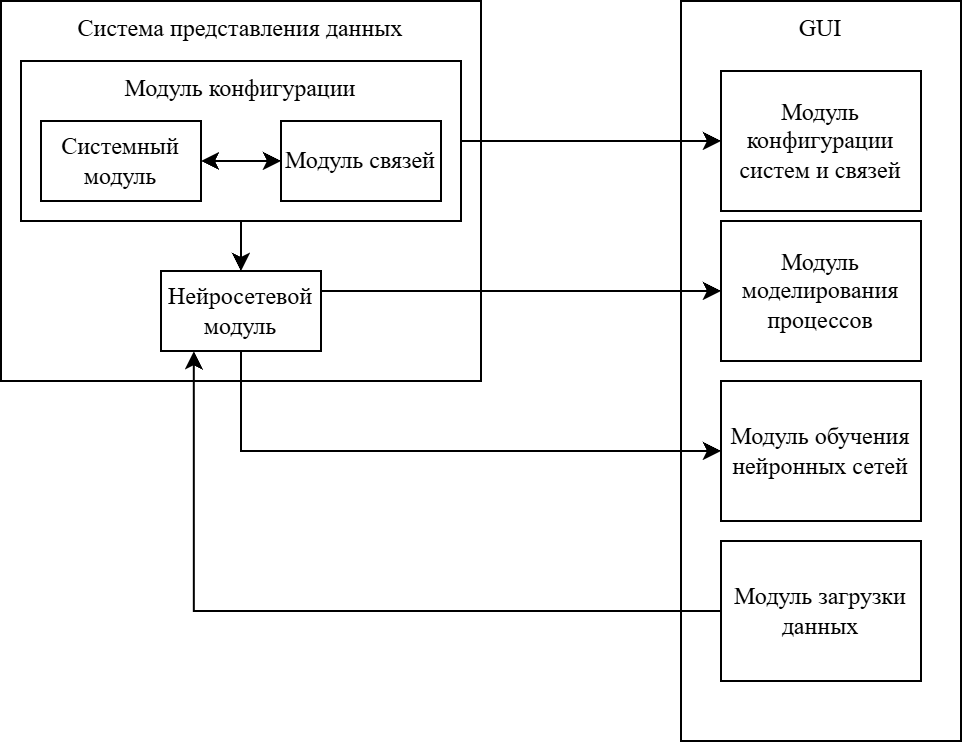
\includegraphics[width=0.95\textwidth]{figures/modules/relations.png}
  \end{center}
  \caption{Модульные связи приложения}\label{fig:modules:relation}
\end{figure}

В частности, программа состоит из двух компонент (см. рис. \ref{fig:modules:relation}) - модуля представления данных и модуля графического интерфейса. 

Система представления данных содержит модуль конфигурации и нейросетевой модуль, реализующий логику поведения систем и их компановку и их идентификацию.

Графический интерфейс реализует модули, позволяющие взаимодействовать с компонентами системы представления и в наглядной форме производить моделирование. 

\subsection{Используемые формы}
%TODO: Перечисление форм и их назначение, какие возможности предоставляют

Графический интерфейс реализует элементы управления и отображения, позволяющие удобно производить процесс динамической идентификации. Приложение состоит из четырех смежных модулей, охватывающих различные области управления и отображения информации:

\begin{itemize}
  \item Модуль загрузки данных;
  \item Модуль конфигурации;
  \item Модуль настройки обучения;
  \item Модуль просмотра и моделирования.
\end{itemize}

\subsubsection{Модуль загрузки данных}

Модель загрузки данных отвечает за загрузку и предварительную обработку экспериментальных данных, необходимых для обучения нейронных сетей каждой подсистемы. 

\begin{figure}[H]
  \begin{center}
    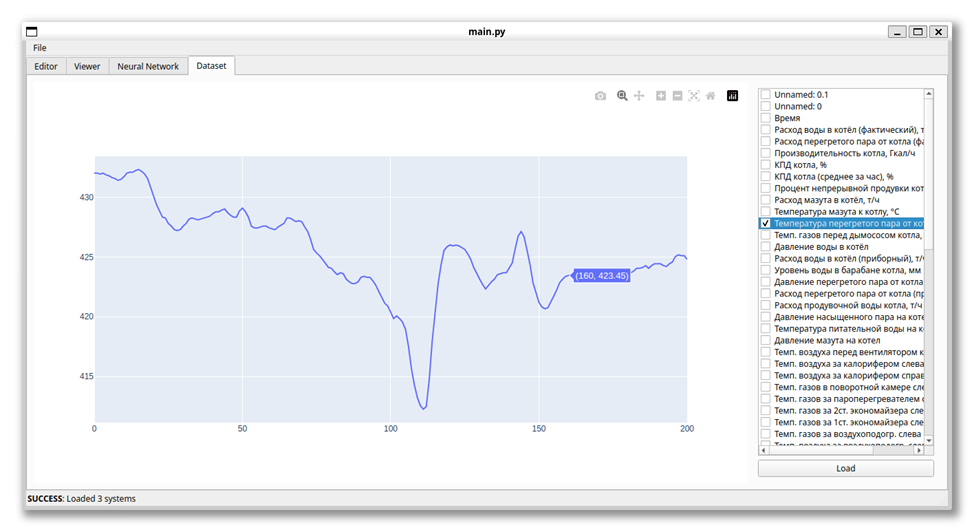
\includegraphics[width=0.95\textwidth]{figures/modules/loader.png}
  \end{center}
  \caption{Форма загрузки и обработки данных}\label{fig:forms:loader}
\end{figure}

\subsubsection{Модуль конфигурации}

Модуль компановки систем и их связей позволяет пользователю определять структуру промышленной установки, указывая конфигурацию подсистемы и сигналы, описывающие поведение системы. 

\begin{figure}[H]
  \begin{center}
    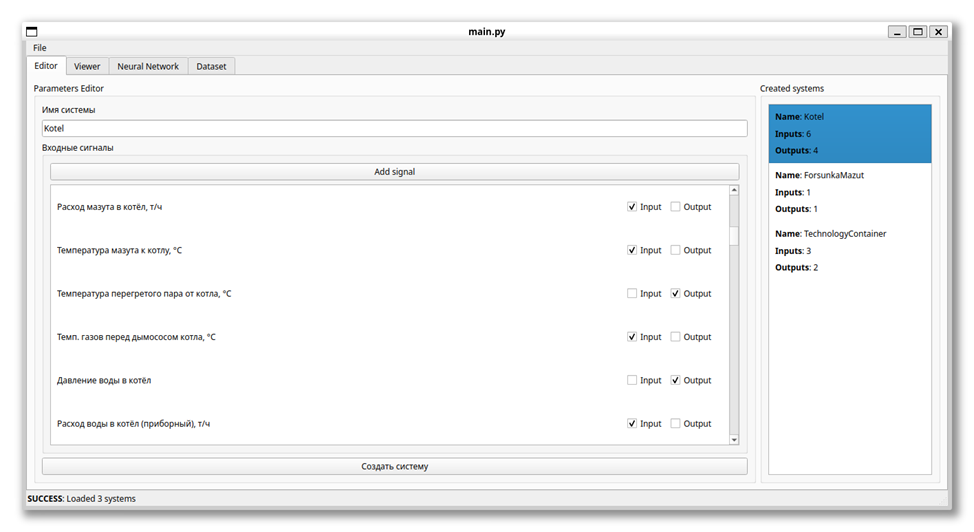
\includegraphics[width=0.95\textwidth]{figures/modules/editor.png}
  \end{center}
  \caption{Форма конфигурации систем и связей}\label{fig:forms:editor}
\end{figure}

\subsubsection{Модуль настройки обучения}

Модуль обучения нейронных сетей реализует возможность задания параметров обучения нейросети, отслеживания процесса обучения нейронных сетей каждой подсистемы на загруженных данных, а также получение отчета об обучении. 

\begin{figure}[H]
  \begin{center}
    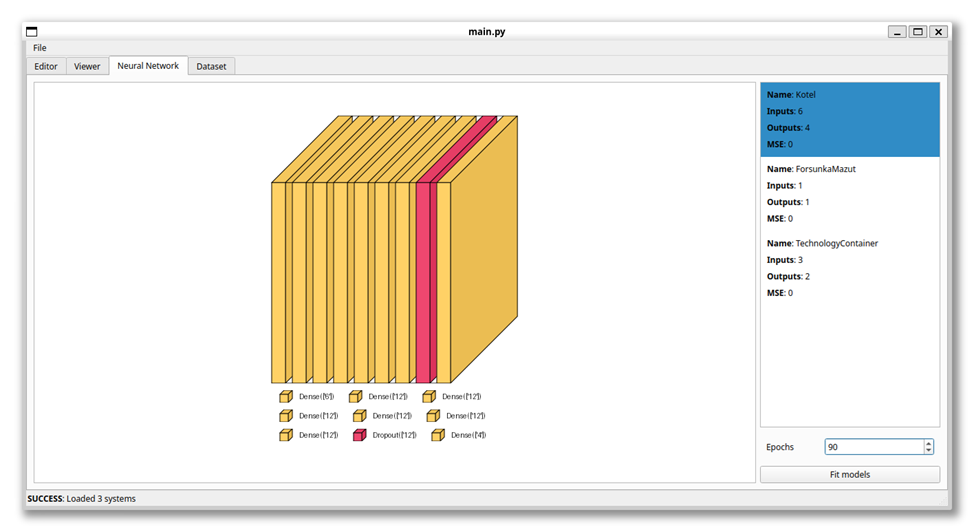
\includegraphics[width=0.95\textwidth]{figures/modules/neural.png}
  \end{center}
  \caption{Форма настройки обучения и структуры нейронных сетей}\label{fig:forms:neural}
\end{figure}

\subsubsection{Модуль просмотра и моделирования}

Модель просмотра скомпонованной системы предоставляет визуальное представление структуры установки с выделением подсистем и связей между ними, а также позволяет пользователю проводить симуляцию поведения идентифицированной системы на основе обученных нейронных сетей. Взаимодействие между этими модулями осуществляется посредством передачи данных через связи подсистем с учетом заданной конфигурации.

\begin{figure}[H]
  \begin{center}
    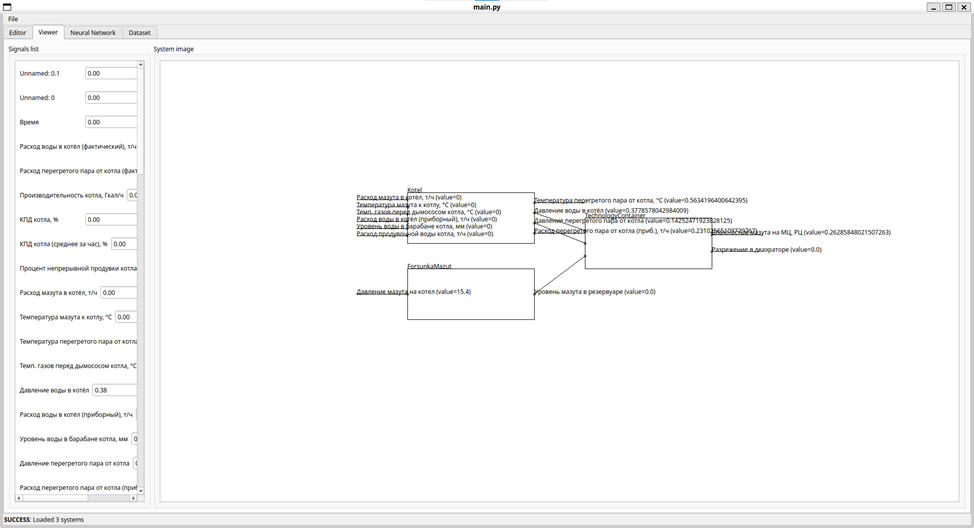
\includegraphics[width=0.95\textwidth]{figures/modules/modelling.png}
  \end{center}
  \caption{Форма просмотра и моделирования}\label{fig:forms:viewer}
\end{figure}

\section{Архитектура связей нейронных сетей}
%TODO: Описать какие модели используются при обучении для описания каждой подсистемы и системы в общем

\section{Оценка работы}
%TODO: Произвести оценку моделирования системы


% Сравнительная часть



\backmatter %% Здесь заканчивается нумерованная часть документа и начинаются ссылки и

Заключение
%% заключение

% Список литературы

% % Список литературы при помощи BibTeX
% Юзать так:
%
% pdflatex rpz
% bibtex rpz
% pdflatex rpz

\bibliographystyle{gost2008}
\bibliography{sections/literature}

%%% Local Variables: 
%%% mode: latex
%%% TeX-master: "rpz"
%%% End:


\appendix   % Тут идут приложения

%
% \include{90-appendix1}
%
% \include{91-appendix2}

\end{document}

%%% Local Variables:
%%% mode: latex
%%% TeX-master: t
%%% End:
